%\doublespacing

\newcommand{\GVL}[1]{{\color{red}\em  GVL: #1}}
\newcommand{\E}[1]{{\color{red}~\blacksquare~\footnote{grammar, spelling, sentence, or other error}~}}

\newcommand{\SHELL}{GridShell}
\newcommand{\AUTHOR}{%
Xi He\\
Rochester Institute of Technology\\
~Bldg 74, Lomb Memorial Drive, Rochester, NY 14623-5608 \\
~xi.he@mail.rit.edu%
}
\newcommand{\TITLE}{The Analysis of A Citation Network Relating to Grid Computing }

%\TABLEOFCONTENTS

\title{\TITLE}
\author{\AUTHOR}

\maketitle

\begin{abstract}
In this study, we analyze a citation network composed of Grid Computing related papers and intent to identify the appropriate literatures for researchers in Grid Computing. We first examine some network characteristics which are effectively used in our network analysis. Then we develop the methodology for network analysis, including modeling methods and data collection process. The experiments are conducted to validate our ideas and detailed interpretations are discussed. Our study shows that it is effective and efficient to find useful literatures for researchers with our analysis methods.
\end{abstract}
\begin{keywords}
Grid Computing, Citation Network, Average Path Length, Cluster Coefficient
\end{keywords}
%%%%%%%%%%%%%%%%%%%%%%%%%%%%%%%%%%%%%%%%%%%%%%%%%%%%%%%%%%%%%%%%%%%%%%
\section{Introduction}
%%%%%%%%%%%%%%%%%%%%%%%%%%%%%%%%%%%%%%%%%%%%%%%%%%%%%%%%%%%%%%%%%%%%%%

In general, the term ``network'' means interconnected system of people or things. A network is composed of a set of connections formed between the individuals in the system to achieve certain goals. For example, Tom has a lot of friends in his Facebook. If we model each of his friends as a node, and use an edge to connect every pair of his friends if they know each other,  a network describing Tom's friends' relationship is formed (Figure \ref{F:facebook}). Some popular networks that are of interest to studies and researches include Computer Network, Communication Network, Financial Network, Social Network and so on.  Networks exist almost everywhere in our world, and have a significant influence on every aspect of our lives.  

\begin{figure}[ht!]
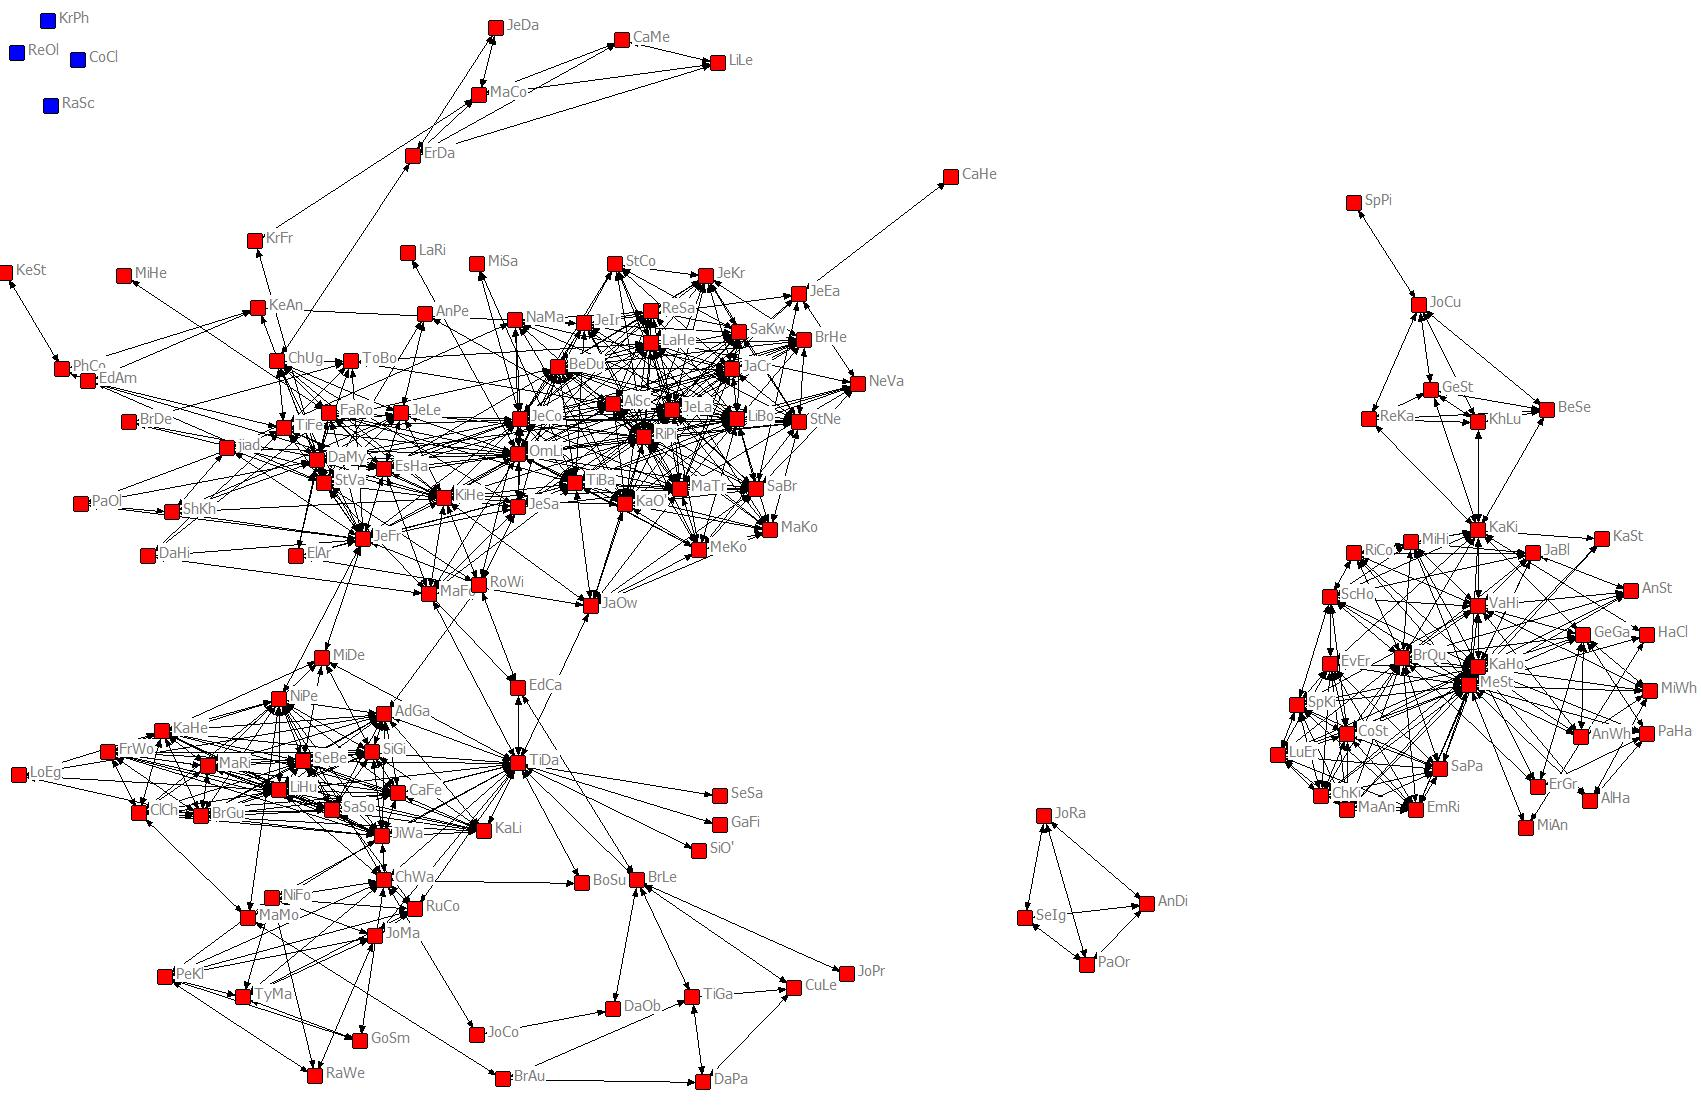
\includegraphics [totalheight=0.23\textheight]{images/facebook.jpg}
\caption {A Facebook Network}
\label {F:facebook}
\end{figure}

The development of network theory, namely the analysis of general networks, has a long history. In 1736, Swiss mathematician Leonhard Euler 	presented his solution to Seven Bridges of K\"{o}nigsberg problem in his paper {\em Seven Bridges of K\"{o}nigsberg}\cite{www-graph}. This event is widely regarded as the beginning of graph theory. After that, graph theory boomed with the contribution from mathematical giants such as Cauchy, Hamilton, Cayley and Kirchhoff. Two century later, Paul Erd\H{o}s and Alfr\'{e}d R\'{e}nyi introduced random network theory in their paper {\em On Random Graphs}\cite{www-random}. Unlike graph theory which aims to discover and catalogue the properties of the various graphs, random network theory tries to answer such questions as how real networks form and what are the laws governing their appearance and structure. Paul Erd\H{o}s and Alfr\'{e}d R\'{e}nyi viewed networks and the world they represented as fundamentally random.  They believe that a network is obtained by starting with a set of n vertices and adding edges between them at random. In 1998, Duncan Watts and Steven Strogatz identified small world networks as a class of random networks\cite{www-small}. Purely random graphs, built according to  Paul Erd\H{o}s and Alfr\'{e}d R\'{e}nyi's theory, exhibit a small average shortest path length along with a small clustering coefficient. Duncan Watts and Steven Strogatz measured that many real-world networks have a small average shortest path length, but also a clustering coefficient significantly higher than expected by random chance. They then proposed a novel network model, which we today call {\em Watts and Strogatz model}. A year later, Albert-L\'{a}szl\'{o} Barab\'{a}si and his colleagues found that some Web nodes, which they called "hubs", had many more connections than others and that the network as a whole had a power-law distribution of the number of links connecting to a node\cite{www-scale}. Albert-L\'{a}szl\'{o} Barab\'{a}si and collaborators coined the term ``scale-free network'' to describe the class of networks that exhibit a power-law degree distribution. 


Today network theory  is an area of computer science, network science and part of graph theory, and is applied in many disciplines including particle physics, computer science, biology, economics and sociology. Its topics include

\begin {itemize}
\item Network theorems: Max flow min cut theorem; Menger's theorem; Metcalfe's law.
\item Network properties: Betweenness; Centrality; Closeness.
\item Network theory application.
\item Networks with certain properties: Complex network, Scale free network, small world network. 
\end {itemize}

The subject of this study is a citation network. With the assistance of network theory, the study can analyze network's properties and their implication. The remainder of the paper is organized as follows. In Section \ref{S:Background}, some network characteristics adopted in our study are thoroughly examined, followed by an introduction to the basic concept of Grid Computing and the motivation for this study in Section \ref{S:Motivation}. Then we introduce the methodology for this study in Section \ref{S:Methodology}. A discussion of the network modeling method and the network simulations adopted in this study is presented.  In the next section, we show the result of the experiments and discuss their implication.  Later the significance and limitations of the study is described in Section \ref{S:Significance}, followed by Section \ref{S:Conclusion} which is the conclusion. 

%%%%%%%%%%%%%%%%%%%%%%%%%%%%%%%%%%%%%%%%%%%%%%%%%%%%%%%%%%%%%%%%%%%%%%
\section{Background \label{S:Background} }
%%%%%%%%%%%%%%%%%%%%%%%%%%%%%%%%%%%%%%%%%%%%%%%%%%%%%%%%%%%%%%%%%%%%%%
The section aims to provide the necessary background for this study. We give a brief introduction of  some network characteristics such as average path length and clustering coefficient. These are the essential statistical metrics for the analysis of the citation network.  We also introduce centrality measurement, an important metrics for measuring the importance of vertices in the networks.

\subsection{Average Path Length}
Average path length is defined as the average number of steps along the shortest paths for all possible pairs of network nodes\cite{www-apl}. 
\\
\begin{equation}
L=\frac{1}{\frac{1}{2}N(N+1)}\sum_{i>=j}d_{ik}
\end{equation}
Where $N$ is the number of nodes, $d_{ik}$ is the distance between two nodes.
\\
Average path length is a measure of the efficiency of information or mass transport on a network.The famous six degrees of separation theory\cite{www-sds} says that if a person is one step away from each person they know and two steps away from each person who is known by one of the people they know, then everyone is at most six steps away from any other person on Earth (See Figure \ref{F:six}). In that case, six is the measurement of efficiency of information transport on the human network.

%In fact, six degrees of separation phenomenon does not limit to human network. For example, Albert-L\'{a}szl\'{o} Barab\'{a}si and his colleagues predicted that the diameter of the Web is 18.59, close to 19. That is, a web page is on average only 19 clicks away from other web pages.


\begin{figure}[ht!]
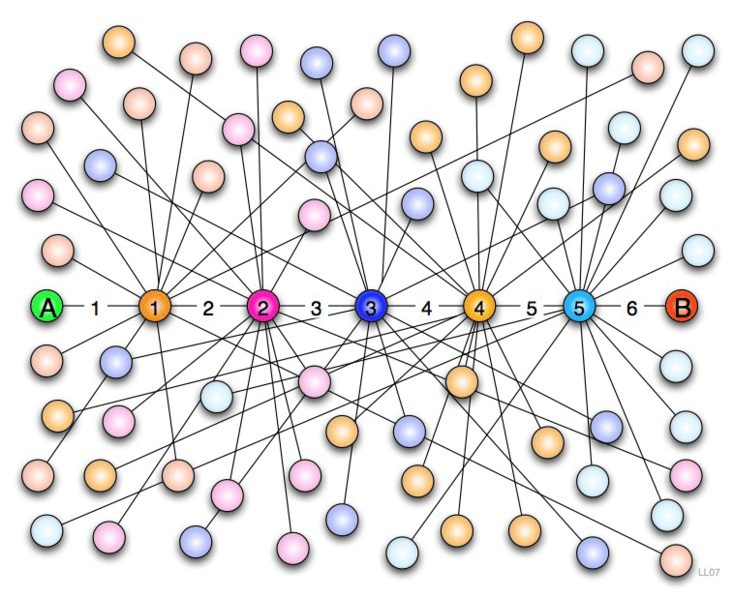
\includegraphics [totalheight=0.3\textheight]{images/six.png}
\caption {Six degrees of separation\cite{www-sds}}
\label {F:six}
\end{figure}



\subsection{Clustering coefficient}
The clustering coefficient of a vertex in a graph quantifies how close its neighbors are to being a clique\cite{www-small}. 

\begin{equation}
C_i=\frac{2E_i}{k_i(k_i-1)}
\end {equation}
Where $E_i$ is the number of edges among the neighbors of node $i$ and $k_i$ is the node $i$'s degree. 

Let us take an example to explain the concept of clustering coefficient. Jack has four friends. If his friends are all friends with each other as well, each of them can be connected with a link. But chances are that some of his friends are not friends with each other. Let us say there are only three links between his friends, few than six links. So the clustering coefficient for Jack's friend cycle is $0.5$. The clustering coefficient tells about how closely the cycle of Tom's friends is. If the clustering coefficient is 1, it means that all of his friends are good friends with each other. On the other hand, if the clustering coefficient is zero, Tom would the only person who hold his friends together.

\subsection{Centrality measurement}

Centrality of a vertex within a graph determines the relative importance of a vertex within the graph\cite{www-centrality}. For example, how important a person is within a social network, or how important a room is within a building. Four kinds of centrality measurement is widely used in network analysis: degree centrality, betweenness, closeness and eigenvector centrality.

\subsubsection{Degree centrality}
Degree centrality is defined as the number of links incident upon a node. Degree is often interpreted in terms of the immediate risk of node for catching whatever is flowing through the network. If the network is directed, then we usually define two separate measures of degree centrality, namely indegree and outdegree. Indegree is a count of the number of ties directed to the node, and outdegree is the number of ties that the node directs to others.
\subsubsection{Betweenness centrality}
Betweenness is a centrality measure of a vertex within a graph. Vertices that occur on many shortest paths between other vertices have higher betweenness than those that do not.
\subsubsection{Closeness centrality}
Closeness centrality represents how far a vertices is from all other vertices in the network. Closeness centrality is based on the concept of network paths. Vertices that tend to have short geodesic distances to other vertices with in the graph have higher closeness.
\subsubsection{Eigenvector centrality}
Eigenvector centrality is a measure of the importance of a node in a network. It assigns relative scores to all nodes in the network based on the principle that connections to high-scoring nodes contribute more to the score of the node in question than equal connections to low-scoring nodes.

%%%%%%%%%%%%%%%%%%%%%%%%%%%%%%%%%%%%%%%%%%%%%%%%%%%%%%%%%%%%%%%%%%%%%%
\section{Motivation \label{S:Motivation}}
%%%%%%%%%%%%%%%%%%%%%%%%%%%%%%%%%%%%%%%%%%%%%%%%%%%%%%%%%%%%%%%%%%%%%%
Grid Computing is a form of distributed computing paradigm originated in the early 1990's in lan Foster's and Carl Kesselman's seminal work: ``The Grid: Blueprint for a new computing infrastructure". Ever since then, Grid Computing has been regarded as one of the hottest research fields in the world. The basic idea of Grid Computing is to combine computer resources from multiple administrative domains, and then apply the powerful computation ability to the scientific, technical or business problems that requires a great number of computer processing cycles or needs to process large amounts of data. Through a decade's development, Grid Computing is mature and well developed. Every aspect of Grid Computing, such as architecture, middleware software, schedule algorithm or performance have been thoroughly studied. At the same time, Grid Computing is also widely applied to or combined with other technologies, and forms plenty of cross-discipline researches.   
%\begin{figure}[ht!]
%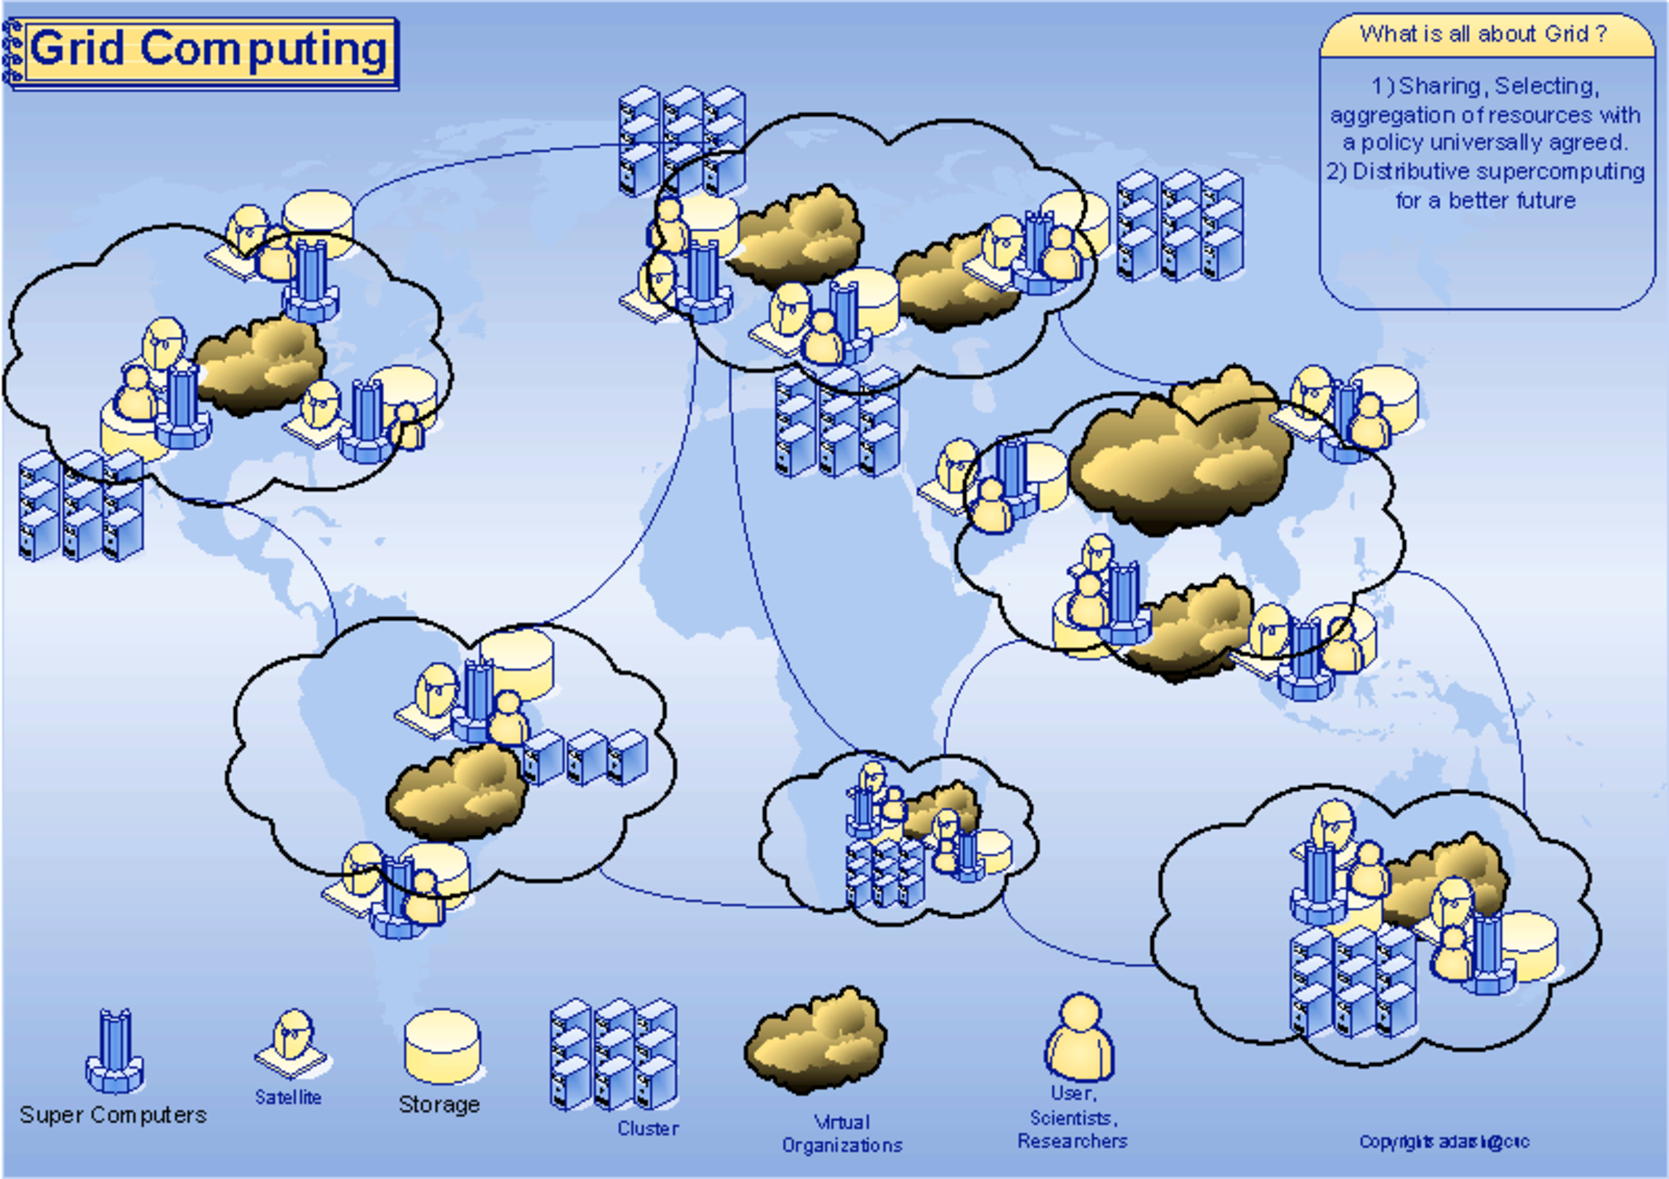
\includegraphics [totalheight=0.25\textheight]{images/gridcomp}
%\caption {Grid Computing}
%\label {F:grid}
%\end{figure}


However, these great achievements put a huge challenge on the researchers new in Grid Computing. First, it is not easy to select the literatures of interest from millions academic literatures across various disciplines. For instance, some papers with the title of ``Grid'' might actually talk about the power grid in the electricity industry. What is more, not all of the literatures in Grid Computing are worthy of reading. Some of literatures are good and useful. Unfortunately, much more literatures might not be as good as expected.  Due to the enormous number of the literatures, it is also not realistic to read through all of the literatures in Grid Computing and then identify which ones are good or which ones are bad.  As a result, it becomes extremely important and critical to provide the novices in Grid Computing with a tool to find out the valuable literatures with little effort. 

The purpose of this study is to provide a way or method for students or researchers interested in Grid Computing to locate the classic literatures in a relatively shorter period. With an exhaustive research and study on the Grid Computing related citation network,  we can study every paper's role and impact in the network of academic papers, thus obtaining reasonable clues determining how to select the appropriate papers. Actually, the study of citation networks has been conducted for a while. In \cite{wu2008topology}, the author analyze motif of journal citation networks, citation pattern and develop trends. In \cite{hung2008small}, the author analyze the small world phenomenon in patent citation networks. However, these papers mainly focus on explore the inner principle of specific citation network. The goal of our study is to provide a set of tools or methods to extract information for the citation network and facilitate other research activities. 


%%%%%%%%%%%%%%%%%%%%%%%%%%%%%%%%%%%%%%%%%%%%%%%%%%%%%%%%%%%%%%%%%%%%%%
\section{Methodology \label{S:Methodology}}
%%%%%%%%%%%%%%%%%%%%%%%%%%%%%%%%%%%%%%%%%%%%%%%%%%%%%%%%%%%%%%%%%%%%%%
In this section, we describe the methodology adopted in the study of Grid Computing related citation network.  Three steps are involved in our study:
\begin{itemize}
\item Network modeling
\item Data collection
\item Data analysis
\end{itemize} 
Below we will describe in detail the process of each step.
\subsection{Network modeling}
First we would model the citation network. We define the Grid Computing related citation network as follows: each paper is regarded as a node, and the citation relationship between papers is represented using arcs. For example, if a paper $B$ cited another paper $A$, we add an arc starting from $B$ and ending at $A$ (See Figure \ref{F:model}).  So the number of arc starting from $B$ represents the number of papers that $B$ cited and the number of arc ending at $A$ stands for the number of papers in which $A$ is cited. In addition, it is almost impossible that a cycle is formed in a citation network. A paper can be cited only when it is published and thus its publishing date is earlier than those citing it. So it can not cite other papers that already cited it so that a cycle is not supposed to appear in the citation network. In fact, a citation network is modeled as a DAG (Directed Acyclic Graph). 

\begin{figure}[ht!]
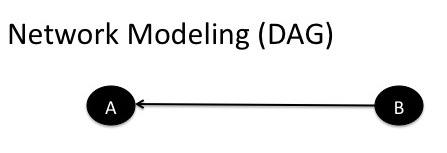
\includegraphics [scale=0.60]{images/model.jpg}
\caption {A network model}
\label {F:model}
\end{figure}

\subsection{Data Collection}

Now that we have a network model, we can collect real data  from the Internet and fit those collected data into our model. 
$CiteSeer^X$ ({\em http://citeseerx.ist.psu.edu/}) is a famous scientific literature library and search engine that focuses primarily on the literature in computer and information science. One of its feature is that it provides a lot of metadata and related services for scientific literature, such as citation statistics and reference linking. So $CiteSeer^X$ is an appropriate candidate as the data source for our study. Grid Computing started in 1990's and has been one of the hottest research topics in the academic community.  As a result, there exists thousands of Grid Computing related papers in $CiteSeer^X$. Due to the limitation of time and resources, our study can only extract a little part of these papers and analyze their citation network. In the process of data collection, we make two assumption. First, we assume that most of the grid related papers has the keyword ``grid'' in their title. Second, we believe that the more an article is cited, the more important the article is to the development of Grid Computing. Following our assumption, we collected a sample of 52 papers which is representative of a whole set of Grid Computing related paper.  The following is the steps of data collection:
\begin{itemize}
\item Search for the papers with the title containing the keyword {\em grid} in $CiteSeer^X$. 
\item Sort the search result in the descending order of number of citations. 
\item Pick out the papers that obviously do not belong to Grid Computing. 
\end{itemize}  

%\begin{figure*}[ht!]
%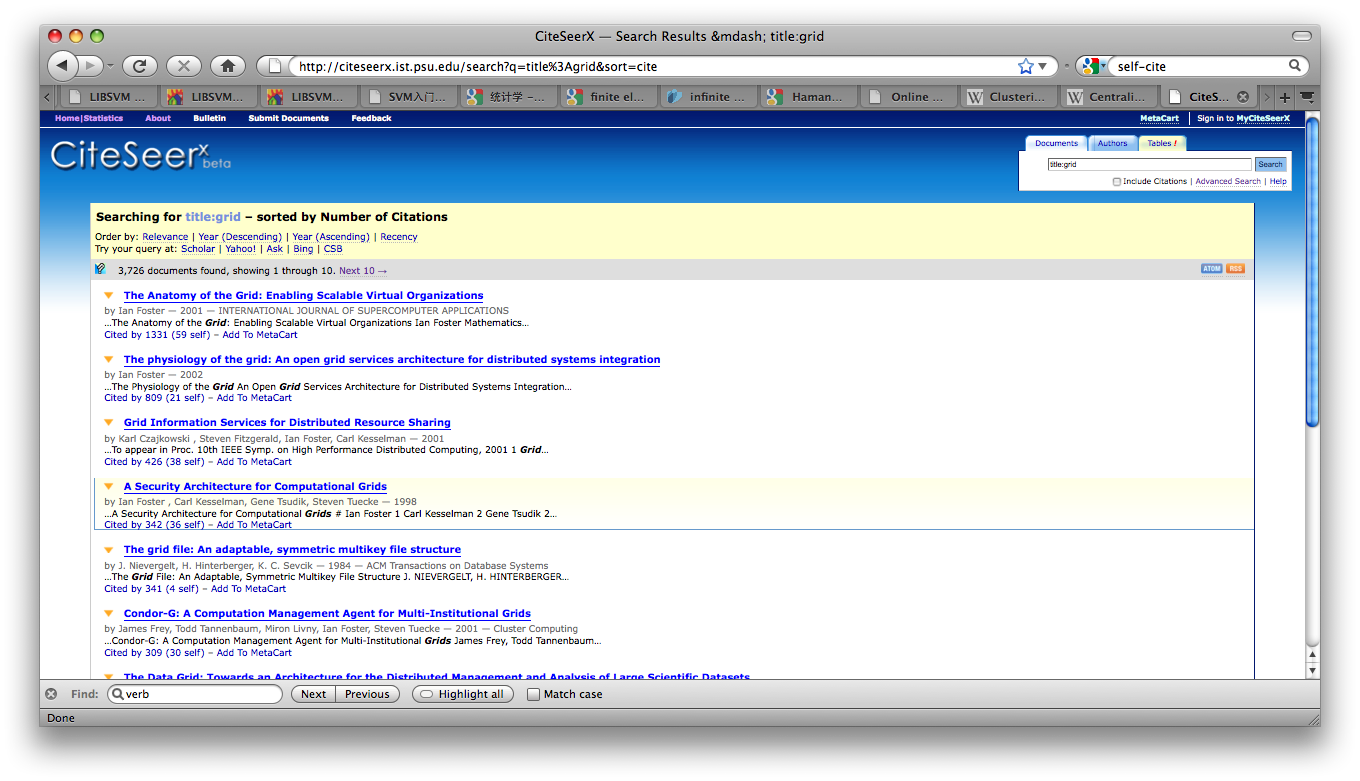
\includegraphics [totalheight=0.4\textheight]{images/citeseer}
%\caption {Search papers with title of ``grid'' in $CiteSeer^X$ }
%\label {F:citeseer}
%\end{figure*}

Table \ref{T:name} lists the title, label and the number of citation of 10 most cited papers in our data collection.
\begin{table}[htb]
\begin{center}
\begin{small}
\begin {tabular} {|p{5.5cm}|c|c|}
\hline 
{\em \bf ~~~~~~~~~~~~~~~~~~~~~~Title} & {\em \bf Label} &{\em \bf Citation}\\
\hline
\hline
The Anatomy of the Grid: Enabling Scalable Virtual Organizations & 001&1327 \\
\hline
The physiology of the grid: An open grid services architecture for distributed systems integration & 002&811 \\
\hline
Grid Information Services for Distributed Resource Sharing  & 003&425 \\
\hline
A Security Architecture for Computational Grids  & 004&343 \\
\hline
Condor-G: A Computation Management Agent for Multi-Institutional Grids & 005&309 \\
\hline
The Data Grid: Towards an Architecture for the Distributed Management and Analysis of Large 
Scientific Datasets & 006&297 \\
\hline
Nimrod/G: An architecture for a resource management and scheduling system in a global computational Grid & 007&212 \\
\hline
High Performance Parametric Modeling with Nimrod/G: Killer Application for the Global Grid & 008&176 \\
\hline
The Grid: Blueprint for a Future Computing Infrastructure & 051&1076 \\
\hline
Globus: A Metacomputing Infrastructure Toolkit& 052&1240 \\
\hline
\end {tabular}

\end{small}
\caption{ 10 Most Cited Papers In Grid Computing}
\label {T:name}
\end{center}
\end {table}
~\\
\subsection{Network analysis}
Traditionally, researchers can gain an understanding of the small networks only with their eyes. However, for the large networks like the social networks, researchers would prefer using statistical methods to explore the networks' statistical properties and their implication with the help of computers.

Pajek \cite{batagelj1998pajek} is a program for analysis and visualization of large networks. It has been widely used as an efficient analysis tool in all kinds of networks, such as social networks, Internet and ISP networks. Pajek provides a wide range of powerful functionalities for network analysis while it is very easy to install and use. Also it is freely available for noncommercial use. All these are the reasons why we choose Pajek as our analysis tool.  

%In Pajek, six types of objects are used and each type of objects has its input file format. These objects and their corresponding input file extension is as follows:
%\begin{itemize}
%\item Network: Vertices and lines. (.net)
%\item Partition: nominal or ordinal properties of vertices. (.clu)
%\item Vector: Numerical properties of vertices. (.vec)
%\item Cluster: Subset of vertices. (.cls)
%\item Permutation: Reordering of vertices. (.per)
%\item Hierarchy: General tree structure on vertices. (.hie)
%\end{itemize} 

%Pajek also provides a large set of functionalities that facilitate and simplifies network analysis. The citation network we are studying belongs to Pajek's network object. A list of functionality aiming at network object is as follows: 

The following are the functionalities in Pajek that can facilitate and simplify network analysis.
\begin{itemize}
\item Manipulate the network. Add, delete and modify the vertices and lines in the network;
\item Retrieve general information about the network. Such as the number of vertices, the number of arcs, edges and loops, density of lines, average degree and so on;
\item Path. Shortest paths, all paths between two vertices;
\item Reordering. Topological ordering, Richchards's numbering, depth/breadth first search;
\item Flows. Maximum flow between two vertices;
\item Critical paths;
\item Visualization;
\end{itemize}

With the assistance of Pajek, we can analysis the citation network from different perspectives with a little bit learning curve. Otherwise, we would have to program to implement the functionality we need, which is much more time-consuming. The following steps show how we use Pajek to facilitate our study.

\paragraph{Installation}
For this study, we use Microsoft Windows XP Professional platform. Download pajek125.exe from {\em http://pajek.imfm.si/doku.php?id=download} and run the installation program.
\paragraph{Data input}
Pajek requires the input file to conform to the special format. We have to make up the input file manually.   
\paragraph{Visualization}
Visualizing the citation network.



%%%%%%%%%%%%%%%%%%%%%%%%%%%%%%%%%%%%%%%%%%%%%%%%%%%%%%%%%%%%%%%%%%%%%%
\section{Experiment and Result \label{S:Result}}
%%%%%%%%%%%%%%%%%%%%%%%%%%%%%%%%%%%%%%%%%%%%%%%%%%%%%%%%%%%%%%%%%%%%%%
\subsection{General Information}

\begin{figure*}[ht!]
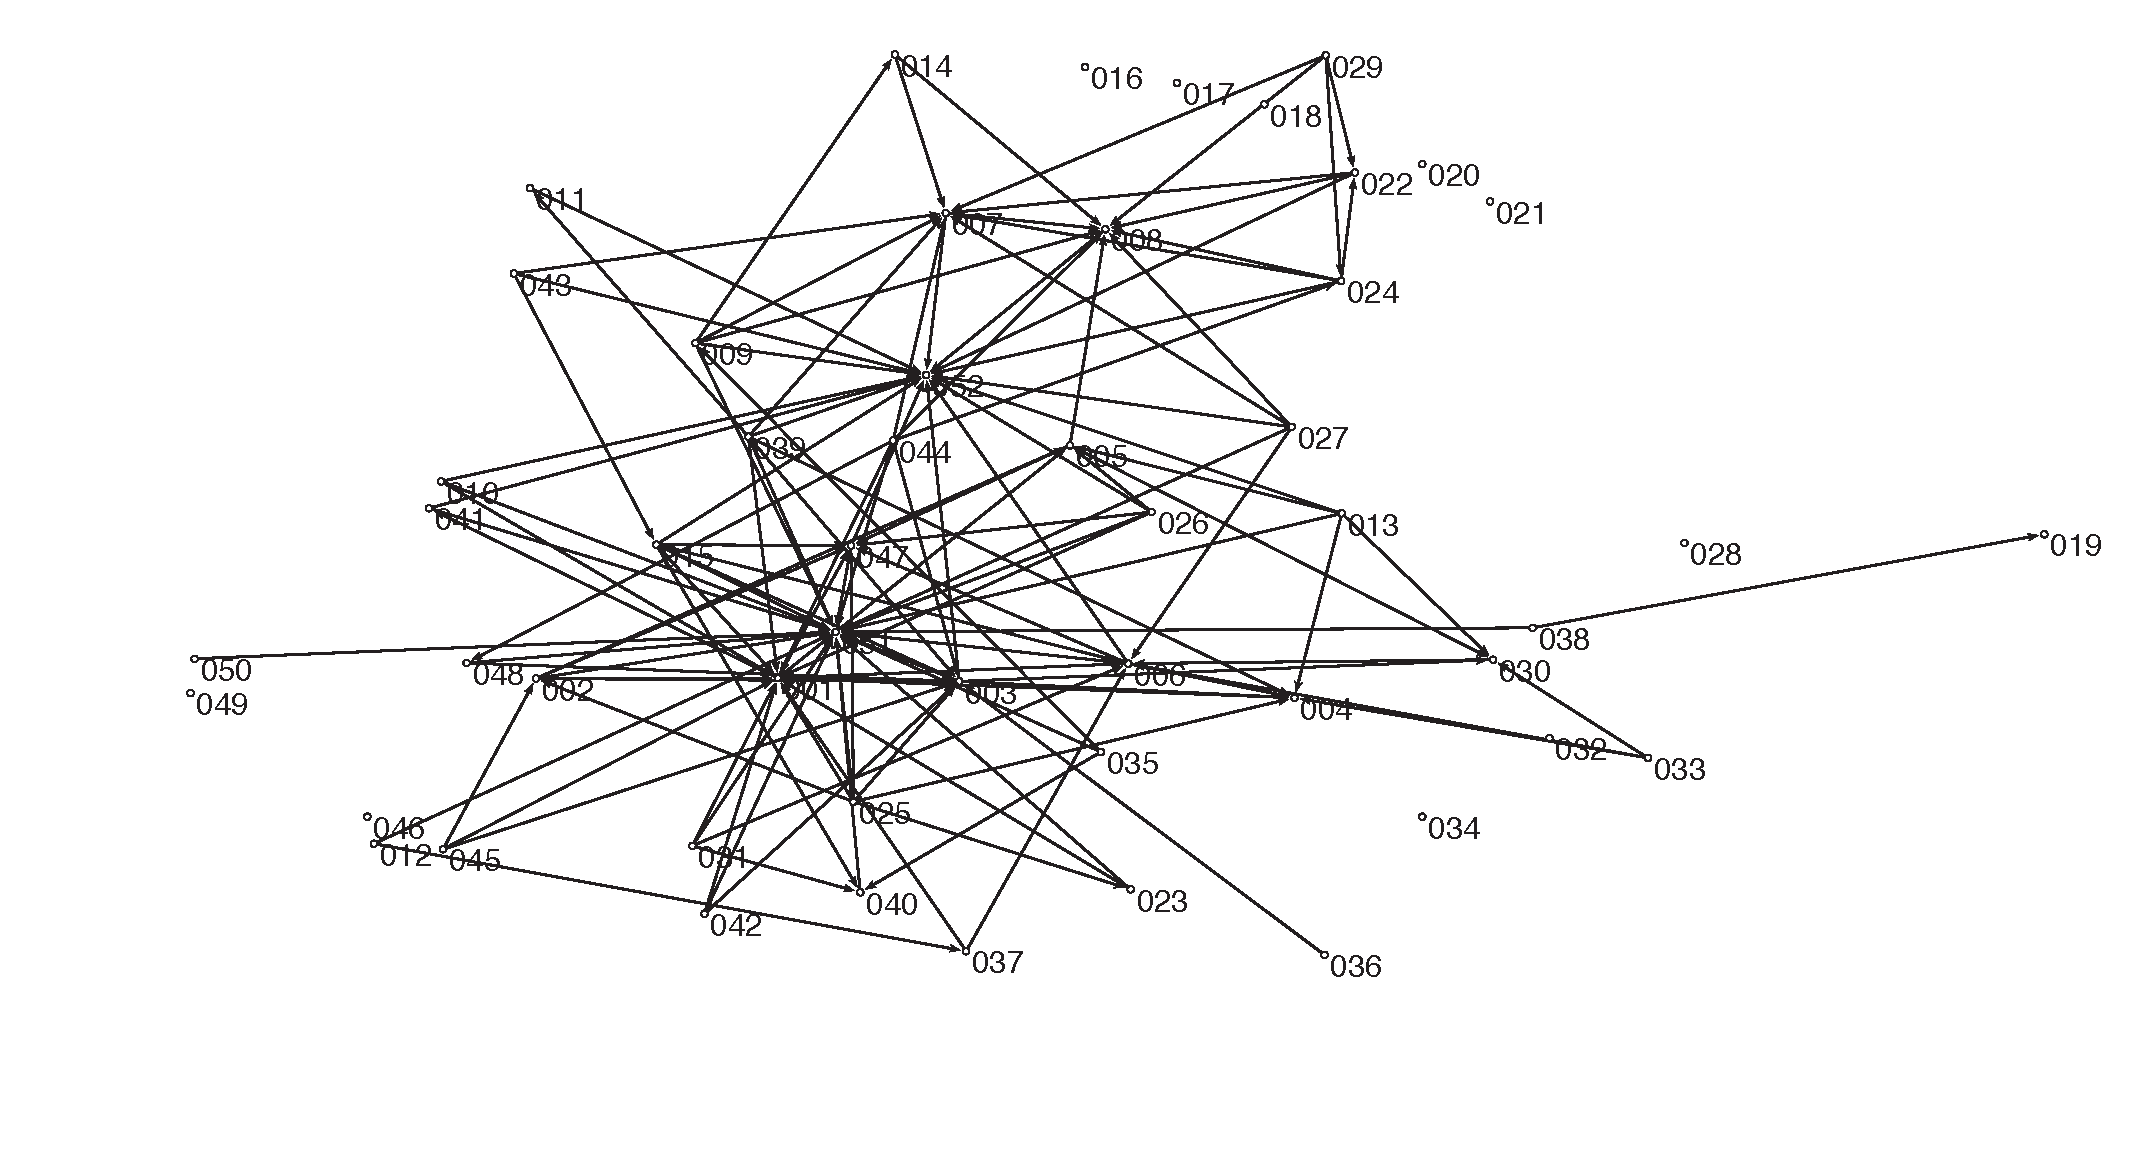
\includegraphics [scale=0.6]{images/citation1}
\caption {Visualization of the citation network}
\label {F:graph}
\end{figure*}

Let us first give an overview of the citation network. Figure \ref{F:graph} is the visualized citation network. We notice that not all the vertices are connected and there are a few vertices acting as a hub and linking to many other vertices. Table \ref{T:papersname} lists the related statistic information. The citation network has 52 nodes and 128 edges; On average each node has 2.56 edges, which means each paper cite or is cited 2.56 times; The maximum in-degree of 24 and out-degree of 7 shows the maximum times a paper is cited or cited other papers; The network diameter is 4, indicating that there are at most 4 nodes at the shortest path of every pair of nodes. The average path length is 1.69, which is small. Therefore we consider the citation network is a small world network. This conclusion is also understandable since researchers in Grid Computing often have strong connections with others and they collaborate with each others in many research activities, which is reflected in their papers.

\begin{table}[htb]
\begin{center}
\begin {tabular}{|c|c|}
%{\em \bf } & {\em \bf Citation}\\
\hline
{\bf ~~~~~~~~Node number~~~~~~~~} & ~~~~~~~~52~~~~~~~~ \\
\hline
{\bf Link Number} & 128 \\
\hline
{\bf Radio L/N}& 2.46 \\
\hline
{\bf Maximum in-degree} & 24 \\
\hline
{\bf Maximum out-degree} & 7\\
\hline
{\bf Network diameter} & 4 \\
\hline
{\bf Average path length}& 1.69 \\
\hline
\end {tabular}
\caption{General Information}
\label {T:papersname}
\end{center}
\end {table}

\subsection{Weakly Connected Subgraphs}
As a complement to the keyword searching strategy adopted in the process of the data collection, we leverage the power of a depth first search (DFS) on the citation network and filter the papers we are not interested in.  Our assumption is that the papers closely related to Grid Computing should be in a weakly connected graph. And by ways of DFS on the citation network, we can identify different weekly connected subgraphs and thus divide the citation network into a handful of subgraphs. The result (Table \ref{T:subgraph}) shows that there are 10 weakly connected subgraphs in our citation network. The biggest subgraph contains 33 vertices while each of the other 9 subgraphs has only one vertex. We notice that the subgraph with 33 vertices represents the mainstream research progress in Grid Computing since many classic papers, such as \cite{Foster01theanatomy},\cite{foster2004grid},\cite{Foster02thephysiology} are included in this subgraph. We also find out that  the papers in the other subgraphs either have nothing to do with Grid Computing or just are little related to Grid Computing and primarily focus on other research topics. So we can pay less attention to or just skip these papers. Above experiment result shows that DFS is a useful tool for filtering papers. 

\begin{table}[htb]
\begin{center}
\begin {tabular} {|c|c|}
\hline
{\em \bf Seq} & {\em \bf Papers in each subgraph}\\
\hline
\hline
1&016\\
\hline
2&017\\
\hline
3&018\\
\hline
4&020\\
\hline
5&021\\
\hline
6&028\\
\hline
7&034\\
\hline
8&046\\
\hline
9&049\\
\hline
%10&001 002 003 004 005 006 007 008 009 010 011 012 013 014 015 019 022 023 024 025 026 027 029 030 031 032 033 035 036 037 038 039 040 041 042 043 044 045 047 048 050 051 052 \\
10&other 33 nodes\\
\hline
\end {tabular}
\caption{ A list of weakly connected subgraphs}
\label {T:subgraph}
\end{center}
\end {table}

\subsection{Directed Acyclic Graph}
\begin{figure}[ht!]
\includegraphics [scale=0.5]{images/loop1}
\caption {Two papers cited each other}
\label {F:loop1}
\end{figure}
Now that we have collected many important papers from the Internet, we would like to verify the validity of these papers before further exploration. Generally speaking, a citation network should be a directed acyclic graph. But in case of wrong data or other reasons, a loop can still be formed in the citation network. Our goal here is to find out the potential loops in the citation network and try to interpret their forming. 

So we conducted a topological sorting on the citation network, and surprisingly, we do find a loop in our citation network. As we can see in Figure \ref{F:loop1}, paper 001 \cite{Foster01theanatomy}  and paper 005 \cite{Frey01condor} cited with each other. However, with thorough investigation, we find out that the fact that two papers cited with each other is caused due to their multiple publishing. As illustrated in Figure \ref{F:loop2},  paper 001's first publishing version does not cite paper 005, but its second publishing version does. At the same time, paper 005's second publishing version cited paper 001's second publishing version. So if we collect the second publishing version of both paper 001and paper 005, we will find that these two papers are cited with each other.

\begin{figure}[ht!]
\includegraphics [scale=0.5]{images/loop2}
\caption {The forming of the loop in the citation network }
\label {F:loop2}
\end{figure}

%\begin{table}[htb]
%\caption{ Two papers cited with each other}
%\label {T:loop}
%\begin{center}
%\begin{small}
%\begin {tabular} {|p{2cm}|p{4cm}|p{2cm}|}
%\hline
%{\em \bf Author} & {\em \bf Title}& {\em \bf Publisher}\\
%\hline
%\hline
%Ian T. Foster&The Anatomy of the Grid: Enabling Scalable Virtual Organizations&CCGRID 2001\\
%\hline
%Ian T. Foster&The Anatomy of the Grid: Enabling Scalable Virtual Organizations&CoRR 2001\\
%\hline
%Ian T. Foster&The Anatomy of the Grid: Enabling Scalable Virtual Organizations&Euro-Par 2001\\
%\hline
%James Frey&Condor-G: A Computation Management Agent for Multi-Institutional Grids&Cluster Computing 2001\\
%\hline
%James Frey&Condor-G: A Computation Management Agent for Multi-Institutional Grids&HPDC 2001\\
%\hline
%\end {tabular}
%\end{small}
%\end{center}
%\end {table}

\subsection{In-degree and Out-degree}

Our next step is to conduct a thorough analysis of the citation network. We are especially interested in finding out the literatures which have the most influence on the development of Grid Computing, which is equal to identifying the most important vertices in the network. As introduced in Section \ref{S:Background}, centrality measurement is a typical method of determining the relative importance of a vertex within the network.  

\begin{table}[htb]
\begin{center}
\begin {tabular} {|c|c|c|c|}
\hline
{\em \bf Vertex} & {\em \bf In-degree}&{\em \bf Vertex } & {\em \bf In-degree}\\
\hline
\hline
001 & 14 &002& 2\\
\hline
003& 9&004& 7 \\
\hline
005 & 4 &006& 7\\
\hline
007& 9&008& 9 \\
\hline
009 & 1 &011& 1\\
\hline
014& 1&015& 1 \\
\hline
019 & 1 &022& 2\\
\hline
023&1&024&2 \\
\hline
030 & 4 &037& 1\\
\hline
040&3&041&1 \\
\hline
047 & 7 &048& 1\\
\hline
051&24&052&17 \\
\hline
\end {tabular}
\caption{Vertices's In-degree}
\label {T:indegree}
\end{center}
\end {table}

%\begin{figure}[ht!]
%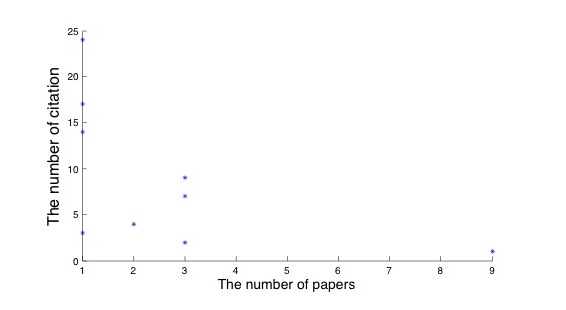
\includegraphics [totalheight=0.25\textheight]{images/indegree}
%\caption {In-degree distribution}
%\label {F:distribution}
%\end{figure}
%
%\begin{table}[htb]
%\begin{center}
%\begin {tabular} {|c|c|c|c|}
%\hline
%{\em \bf Label } & {\em \bf Out-degree}&{\em \bf Label } & {\em \bf Out-degree}\\
%\hline
%\hline
%001 & 14 &002& 2\\
%\hline
%003& 9&004& 7 \\
%\hline
%005 & 4 &006& 7\\
%\hline
%007& 9&008& 9 \\
%\hline
%009 & 1 &011& 1\\
%\hline
%014& 1&015& 1 \\
%\hline
%019 & 1 &022& 2\\
%\hline
%023&1&024&2 \\
%\hline
%030 & 4 &037& 1\\
%\hline
%040&3&041&1 \\
%\hline
%047 & 7 &048& 1\\
%\hline
%051&24&052&17 \\
%\hline
%\end {tabular}
%\caption{ Out-degree distribution of the citation network}
%\label {T:outdegree}
%\end{center}
%\end {table}


In our experiment, we adopt degree centrality, one type of centrality measurement, as our metrics for measuring the importance of the vertices. Table \ref{T:indegree}  lists the in-degree of different vertices in the citation network. We can see that a few vertices have much higher in-degree than others. For example, vertex 051 has a in-degree of 24 and vertex 052 has 17. Table \ref{T:papers}  enumerates three vertices with highest in-degree and their representing literatures. The third column of the table is the number of total citation of these literatures. Every papers in this table has more than 1000 citations, which also prove these papers are extremely important and contribute a lot to the academic community.  Therefore, these papers are worthy of researchers' most attention.

It is very interesting to use betweenness centrality or closeness centrality as another metrics for measuring the importance of the vertices in the citation network. We also expect that the combination of these three metrics can produce more accurate and significant results.

\begin{table}[htb]
\begin{center}
\begin{small}
\begin {tabular} {|c|p{5cm}|c|}
\hline
{\em \bf In-degree} & {\em \bf ~~~~~~~~~~~~Title}&{\em \bf Citation} \\
\hline
\hline
24&The Grid: Blueprint for a Future Computing Infrastructure& 1327\\
\hline
17&Globus: A Metacomputing Infrastructure Toolkit &1076 \\
\hline
14&The Anatomy of the Grid: Enabling Scalable Virtual Organizations&1329\\
\hline
\end {tabular}
\caption{ Papers with high citations}
\label {T:papers}
\end{small}
\end{center}
\end {table}

\subsection{Topological Sorting}
%%%%%%%%%%%%%%%%%%%%%%%%%%%%%%%%%%%%%%%%%%%%%%%%%%%%%%%%%%%%%%%%%%%%%%
Another challenge that researchers are confronted with is that there is no easy way for them to find out how the research in Grid Computing advanced. In other words, they want to know the chains of research development, i.e. one paper is based on which papers.

To address this problem, we propose to conduct a breadth first search (BFS) on the citation network and generate the spanning tree which can be regarded as the research development path. As to different BFS implementation, we might have different development paths. Figure \ref{F:graph} is one possible path. With this path, researchers can have an overview of research progress in Grid Computing. For example, paper 001 originated from paper 051 while it resulted in paper 002. 


\begin{figure}[ht!]
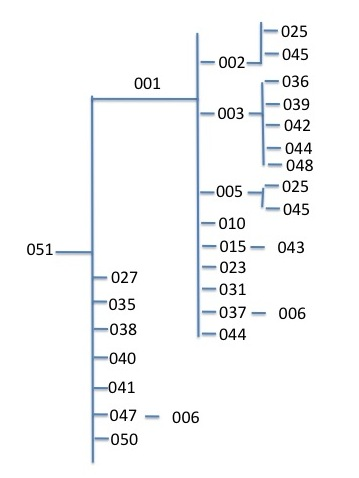
\includegraphics [totalheight=0.5\textheight]{images/structure.jpg}
\caption {Development path of Grid Computing}
\label {F:graph}
\end{figure}

\section{Significance and Limitation \label{S:Significance} }
%%%%%%%%%%%%%%%%%%%%%%%%%%%%%%%%%%%%%%%%%%%%%%%%%%%%%%%%%%%%%%%%%%%%%%
%In this work we aim to find the most useful and classic literatures via the analysis of the citation network. We first exclude literatures unrelated to our theme by means of  dividing the network into a number of weakly connected subgraphs and excluding the subgraphs with little vertices. We also conduct a topological sorting to detect if there exist some cycles in the graph. Then we analyze the in-degree distribution of the network and find a few vertices with extremely high in-degree which we think represent significant literatures.  

In this work we intend to extract useful information for researchers in Grid Computing by means of network analysis. The significance of this work lies in the following aspects:

\begin {itemize}
\item We have a simple but useful citation network model that can be applied to other types of citation networks. Besides, the analysis techniques used in this study can be also applied to other cases of citation network analysis.
\item We have a complete and effective methodology, from network modeling, data collection to network analysis.
\item The analysis methods adopted in the study are innovative. For example, we validate data integrity by conducting a topological sorting. We also derive the research development path in Grid Computing from the spanning trees of the citation network.
\end {itemize}

However, there also exist a few limitations in this paper, including 

\begin{itemize}
\item Due to the limitation of time and resources, the data we collected is limited. We think that the study based on more data would be more significant.
\item As is known to many researchers, self-citation exists widely and these self-citations have little academic implication. We think that our work would be improved if we take the self-citations into consideration in our study.
\end{itemize} 


\section{Conclusion \label{S:Conclusion} }
%%%%%%%%%%%%%%%%%%%%%%%%%%%%%%%%%%%%%%%%%%%%%%%%%%%%%%%%%%%%%%%%%%%%%%
In this study, we conduct a study on a Grid Computing related citation network with the goal of identifying appropriate literatures for researchers interested in Grid Computing. We develop our methodology for network analysis, including modeling methods and data collection process. Based on the methodology, we first exclude literatures unrelated to our theme by means of  dividing the network into a number of weakly connected subgraphs and excluding the subgraphs with little vertices. We also conduct a topological sorting to detect the possible citation cycle. Then we analyze the in-degree distribution of the network and find a few vertices with extremely high in-degree which we think represent significant literatures. Our experiment shows that our methods are feasible.
